%--------------------------------------
% Create title frame
\titleframe

%--------------------------------------
% Table of contents
\begin{frame}[allowframebreaks]{Overview}
  \setbeamertemplate{section in toc}[sections numbered]
  \tableofcontents%[hideallsubsections]
\end{frame}


% What will we learn slide
\begin{frame}{What will we learn today?}
    \small
    Mostly from Chapter 2 of Ned Mohan's book:

    \begin{center}
        Mohan, Ned. Electric power systems: a first course. John Wiley \& Sons, 2012.
    \end{center}

    \begin{itemize}
        \item 3-phase systems
        \item Power transfer between AC systems
        \item Per unit normalization
    \end{itemize}
    You will be able to do exercises 2.1, 2.2, 2.4, 2.5, 2.9, 2.11, 2.12, 2.14, 2.16, 2.17, 2.18, 2.19 and 2.20 from the Ned Mohan's book.
\end{frame}



\section{Three-phase systems (reminder)}
% Three-phase system slide
\begin{frame}{Three-phase system }
Here is an example of a simplified three-phase system with one generator, a transmission line, and a load.
\begin{columns}
    \begin{column}{0.55\textwidth}
    \begin{figure}
        \centering
        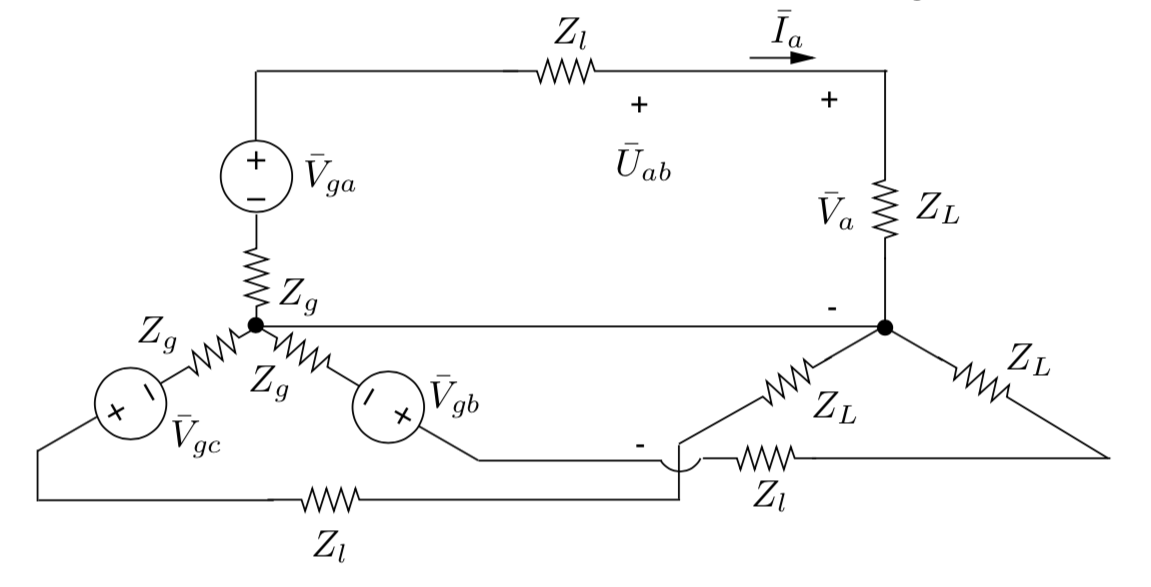
\includegraphics[width=\textwidth]{images/three-phase-system.png}
        \caption{Generation -> transmission -> load}
    \end{figure}
    \end{column}
    \begin{column}{0.35\textwidth}
    Here the load is connected as a \textit{star}. A neutral point is present. 
    
    The neutral conductor is not necessarily implemented, depending on the voltage level and the unbalanced nature of the network.
    \end{column}
\end{columns}
\end{frame}

% Voltage sources slide
\begin{frame}{By design the voltage sources are shifted by 120° and of the same magnitude}
    \begin{columns}
    \begin{column}{0.4\textwidth}
        \begin{align*}
        \bar{V}_{ga} &= V e^{j\phi_u} \\
        \bar{V}_{gb} &= V e^{j(\phi_u - 2 \pi / 3)} = \bar{V}_{ga} e^{-j 2 \pi / 3} \\
        \bar{V}_{gc} &= V e^{j(\phi_u - 4 \pi / 3)} = \bar{V}_{ga} e^{-j 4 \pi / 3}
        \end{align*}

    {\scriptsize In this course, we will always assume that the voltage sources generate a \textbf{positive sequence}, unless explicitly stated.}

    \end{column}
    \begin{column}{0.6\textwidth}
        \begin{figure}
            \centering
            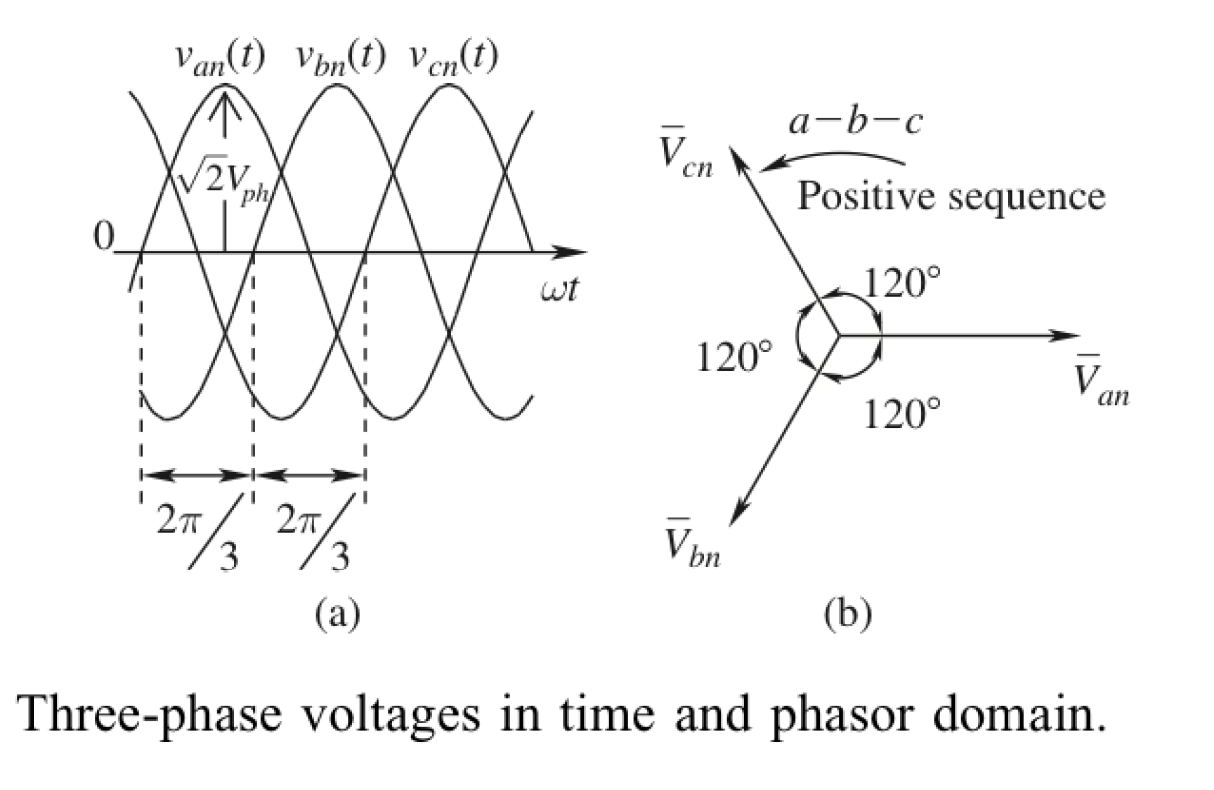
\includegraphics[width=0.99\textwidth]{images/3ph_time_vs_phasor.PNG}
        \end{figure}
    \end{column}
\end{columns}

\end{frame}

% Phase voltage vs line to line voltage slide
\begin{frame}{Phase voltage vs. line to line voltage}

    \begin{columns}
    \begin{column}{0.5\textwidth}
        These voltages represent the \textbf{phase voltages} (between a phase and the ground). If we now look at the \textbf{line to line voltages}:
        $$
        \bar{U}_{ab} = \bar{V}_{ga} - \bar{V}_{gb} = \sqrt{3} \bar{V}_{ga} e^{j\pi / 6}
        $$
        and similarly for $\bar{U}_{bc}$ and $\bar{U}_{ca}$.
    \end{column}
    \begin{column}{0.5\textwidth}
        \begin{figure}
        \centering
        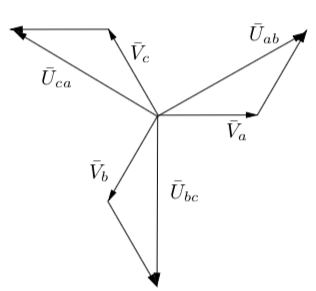
\includegraphics[width=0.6\textwidth]{images/line_vs_phase_voltage_diagram.png}
        \caption{Line vs. phase voltages}
        \end{figure}
    \end{column}
\end{columns}

\textit{Example:} My house is fed by a 400V three-phase system. This means the line voltages are 400V (rms), and thus phase voltages are 230V (approximately). Typically, the phase voltages are distributed independently in the house, each with the neutral.

\end{frame}

% Total power slide
\begin{frame}{Total power}
    The total complex power transmitted to the load is
    $$
    S = \sum_{k \in \{a, b, c\}} \bar{V}_{gk} \bar{I}^*_{k}
    $$
    Hence in a balanced system the total active power to the load is $3VI \cos \phi$, with 3 or 4 wires (instead of 2 in a single-phase system).
\end{frame}


% Comments slide
\begin{frame}{Comments}
    \begin{itemize}
        \item In every phase there is a current flowing. In a balanced system, currents are phase shifted by 120° and sum to zero. Thus the neutral can in theory be removed. This is done in some portions of the global system (typically at high voltage), where neutral points are grounded.
        \item Some loads can also be connected in "delta", hence the neutral is not accessible.
        \item Finally, in unbalanced systems, currents are dictated by the impedances seen in the different phases. There is no perfectly known relation, a priori.
    \end{itemize}
\end{frame}

% Useful formulas slide
\begin{frame}{Useful formulas: from star to delta connection (and back)}
    \begin{figure}
        \centering
        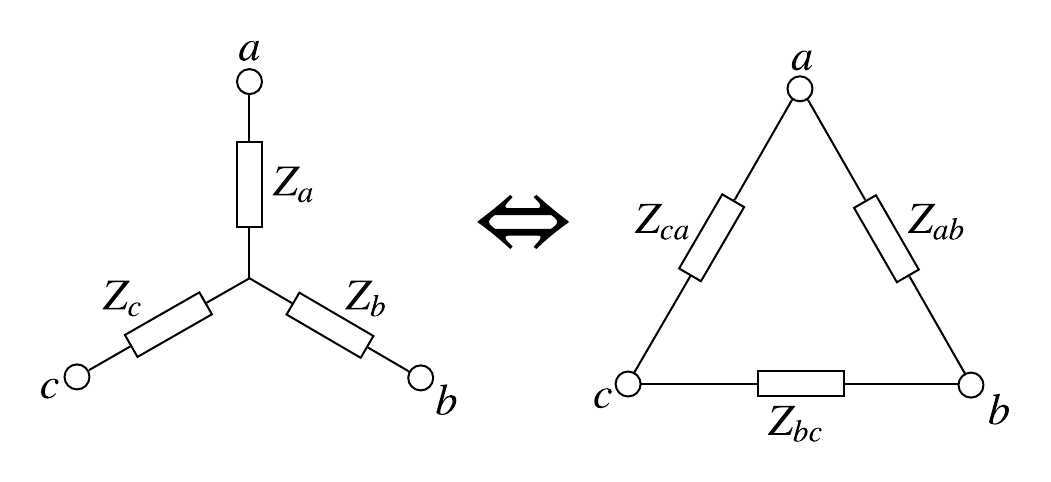
\includegraphics[width=0.5\textwidth]{images/star_delta.png}
    \end{figure}
    \begin{columns}
        \begin{column}{0.5\textwidth}
            $$ \begin{aligned}
            Z_a &= \frac{Z_{ab}Z_{ca}}{Z_{ab} + Z_{bc} + Z_{ca}} \\
            Z_b &= \frac{Z_{bc}Z_{ab}}{Z_{ab} + Z_{bc} + Z_{ca}} \\
            Z_c &= \frac{Z_{ca}Z_{bc}}{Z_{ab} + Z_{bc} + Z_{ca}}
            \end{aligned}$$
        \end{column}
        \begin{column}{0.5\textwidth}
            $$ \begin{aligned}
            Z_{ab} &= \frac{Z_{a}Z_{b}+Z_{b}Z_{c}+Z_{c}Z_{a}}{Z_{c}} \\
            Z_{bc} &= \frac{Z_{a}Z_{b}+Z_{b}Z_{c}+Z_{c}Z_{a}}{Z_{a}} \\
            Z_{ca} &= \frac{Z_{a}Z_{b}+Z_{b}Z_{c}+Z_{c}Z_{a}}{Z_{b}}
            \end{aligned}$$
        \end{column}
    \end{columns}
    What happens in a balanced system?
\end{frame}

% Exercise slide
\section{Neutral break exercise}
\begin{frame}[allowframebreaks]{Neutral break: problem statement}
    Consider a 3-phase Y-connected resistive circuit with unbalanced resistors in the phases. In normal operation there is a neutral wire. Then the neutral breaks (opens).
    \begin{itemize}
        \item Compute in both cases the voltages across the resistors, the currents and the consumed powers.
        \item What can you observe?
    \end{itemize}
    \textbf{Assumptions:}
    \begin{itemize}
        \item 3-phase balanced voltage supply: $U_{ab} = U_{bc} = U_{ca} = U_L$ (line-to-line voltage)
        \item Phase voltages (line-to-neutral) are given by $V_{an} = V_{bn} = V_{cn} = \frac{U_L}{\sqrt{3}}$, and the angle between them is $120^\circ$ (direct sequence).
        \item Unbalanced resistances: $R_a$, $R_b$, $R_c$ (different resistances in each phase).
    \end{itemize}

    \begin{block}{Make a schematic of the two cases (neutral present or absent)}
        \vspace{3cm}
    \end{block}
\end{frame}

% Case 1: Neutral Connected slide
\begin{frame}{Case 1: Neutral Connected}
    \textbf{Voltages:} In normal operation, with the neutral connected, each resistor has its corresponding phase voltage across it:
    $$\bar{V}_{R_a} = \bar{V}_{an}, \quad \bar{V}_{R_b} = \bar{V}_{bn}, \quad \bar{V}_{R_c} = \bar{V}_{cn}$$
    \textbf{Currents:} The current in each phase is given by Ohm's law:
    $$\bar{I}_a = \frac{\bar{V}_{an}}{R_a}, \quad \bar{I}_b = \frac{\bar{V}_{bn}}{R_b}, \quad \bar{I}_c = \frac{\bar{V}_{cn}}{R_c}$$
    The neutral current, $\bar{I}_n$, is the sum of the phase currents:
    $$\bar{I}_n = \bar{I}_a + \bar{I}_b + \bar{I}_c$$
    Due to the unbalanced resistances, $\bar{I}_n$ will not be zero.
\end{frame}

% Powers slide
\begin{frame}{Powers}
    The power consumed in each phase is:
    $$P_a = V_{an} I_a = \frac{V_{an}^2}{R_a}, \quad P_b = \frac{V_{bn}^2}{R_b}, \quad P_c = \frac{V_{cn}^2}{R_c}$$
    Total power consumed:
    $$P_{\text{total}} = P_a + P_b + P_c$$
\end{frame}

% Case 2: Neutral Broken slide
\begin{frame}{Case 2: Neutral Broken}
    When the neutral breaks, the three resistors form a system without a direct connection to the neutral point. The current through each resistor still needs to sum to zero because the current has no return path through the neutral. This changes the voltage distribution across the resistors.
\end{frame}

% Voltages: slide
\begin{frame}[allowframebreaks]{Voltages and currents}
    Here, $\bar{V}_{N'} $ is an unknown voltage offset at the floating point $N'$ (the shifted neutral). 
    
    Since the currents in each phase are given by:
    $$
    \bar{I}_a = \frac{\bar{V}_{aN'}}{R_a}, \quad \bar{I}_b = \frac{\bar{V}_{bN'}}{R_b}, \quad \bar{I}_c = \frac{\bar{V}_{cN'}}{R_c}
    $$
    and, if the neutral is broken, the sum of these currents must equal zero:
    $$
    \bar{I}_a + \bar{I}_b + \bar{I}_c = 0,
    $$
    then 
    \begin{equation}
    \frac{\bar{V}_{aN'}}{R_a} + \frac{\bar{V}_{bN'}}{R_b} + \frac{\bar{V}_{cN'}}{R_c} = 0 \label{eq:neutral_break_KCL}    
    \end{equation}
    that we can now decompose into
    $$
    \frac{\bar{V}_{an}-\bar{V}_{nN'}}{R_a} + \frac{\bar{V}_{bn}-\bar{V}_{nN'}}{R_b} + \frac{\bar{V}_{cn}-\bar{V}_{nN'}}{R_c} = 0 \label{eq:neutral_break_KCL}    
    $$
    which finaly yields
    $$
    \bar{V}_{nN'} \left(\frac{1}{R_a}+\frac{1}{R_b}+\frac{1}{R_c}\right) =     \frac{\bar{V}_{an}}{R_a} + \frac{\bar{V}_{bn}}{R_b} + \frac{\bar{V}_{cn}}{R_c} 
    $$

\end{frame}

% Powers: slide
\begin{frame}{Powers}
    \begin{itemize}
        \item The power consumed in each phase is:
        $$
        P_a = V_{aN'} I_a = \frac{(V_{aN'})^2}{R_a}, \quad P_b = \frac{(V_{bN'})^2}{R_b}, \quad P_c = \frac{(V_{cN'})^2}{R_c}
        $$
        \item Total power consumed:
        $$
        P_{\text{total}} = P_a + P_b + P_c
        $$
    \end{itemize}
\end{frame}

% Observations: slide
\begin{frame}[allowframebreaks]{Numerical example}



With $R_a= 5\Omega$, $R_b= 10\Omega$, $R_c= 20\Omega$ in a 400 V system
    (\href{https://colab.research.google.com/drive/1pXH21c8g9Hv3h94pb81OtuFVQfauG63T?usp=sharing}{\textcolor{blue}{\underline{Link to the Python notebook}}}): 

\begin{center}
    \small
\begin{tabular}{|l|r|r|}
\hline
\textbf{Parameter} & \multicolumn{1}{c|}{\textbf{Case 1: Neutral Connected}} & \multicolumn{1}{c|}{\textbf{Case 2: Neutral Broken}} \\
\hline
\textbf{Total Power (W)} & 18515.00 & 15870.00 \\
\textbf{Phase A Power (W)} & 10580.00 & 4534.29 \\
\textbf{Phase B Power (W)} & 5290.00 & 6801.43 \\
\textbf{Phase C Power (W)} & 2645.00 & 4534.29 \\
\hline
\textbf{Phase A Current (A)} & 46.00 & 30.11 \\
\textbf{Phase B Current (A)} & 23.00 & 26.08 \\
\textbf{Phase C Current (A)} & 11.50 & 15.06 \\
\hline
\textbf{Phase A Voltage (V)} & 230.00 & \alert{150.57} \\
\textbf{Phase B Voltage (V)} & 230.00 & \textcolor{red}{\bf 260.80} \\
\textbf{Phase C Voltage (V)} & 230.00 & \textcolor{red}{\bf 301.14} \\
\hline
\end{tabular}
\end{center}



\end{frame}

\begin{frame}{Observations}
    
    When the neutral is connected, the currents and powers are straightforwardly determined.

    When the neutral is broken, 
    \begin{itemize}
        \item the voltage distribution becomes more complex, and the voltages across the resistors are no longer the same as the phase-to-neutral voltages
        \item Some large overvoltages (equipment might not function as expected) and undervoltages (equipment might be damaged) can appear
        \item the total power consumed changes
    \end{itemize}
\end{frame}



% Per-phase analysis slide
\section{Per-phase analysis}
\begin{frame}[allowframebreaks]{Per-phase analysis}
    In a \textbf{balanced} system, analyses can be simplified by representing only one phase.
    
    This is straightforward if there are no couplings between phases.
    \begin{figure}
        \centering
        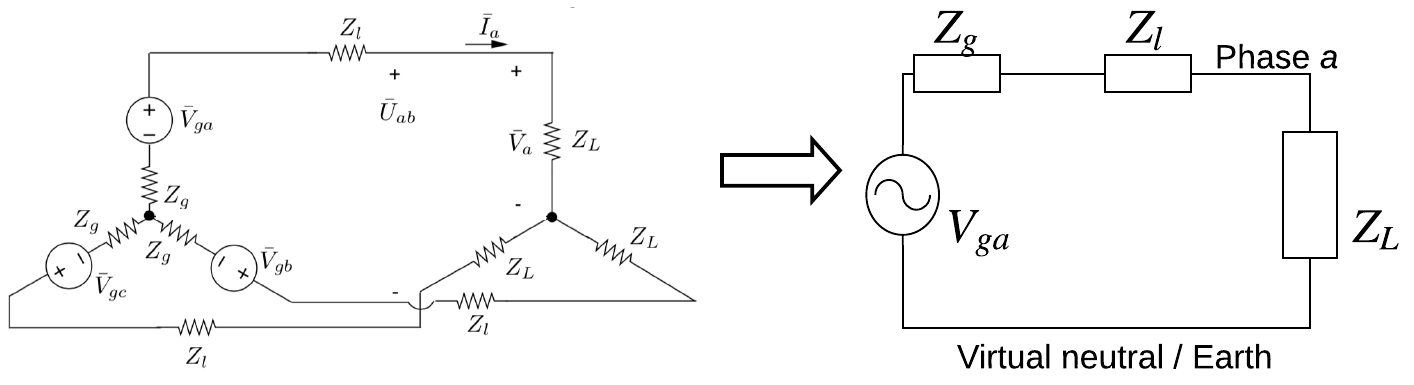
\includegraphics[width=0.8\textwidth]{images/per-phase.png}
    \end{figure}
    In case there is a coupling, and that for instance the voltage drop $\bar{V}_{aA}$ along a line presenting an impedance $Z_{self}$ traversed by a current $\bar{I}_{a}$ is also function of the currents in the other phases:
$$\bar{V}_{aA} = Z_{self} \bar{I}_{a} + Z_{mutual} \bar{I}_{b} + Z_{mutual} \bar{I}_{c}$$
then the per-phase equivalent impedance (for phase $a$) is $$Z_{aA} = Z_{self} - Z_{mutual}$$
since $\bar{I}_{a} + \bar{I}_{b} + \bar{I}_{c} = 0$
\end{frame}

\begin{frame}{One-line diagram}
\begin{figure}
        \centering
        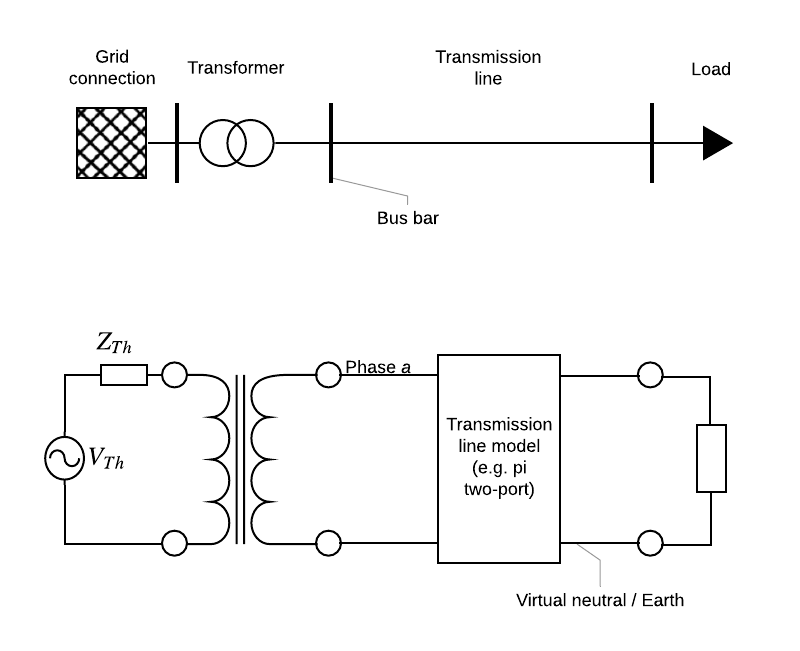
\includegraphics[width=0.6\textwidth]{images/one-line.png}
    \end{figure}
\end{frame}

\section{Power transfer between AC systems}
% Power transfer between AC systems slide
\begin{frame}[allowframebreaks]{Power transfer between AC systems}
    \begin{columns}
        \begin{column}{0.5\textwidth}
            Consider the following simple system. We have $\bar{I} = \frac{\bar{V}_s-\bar{V}_r}{jX}$
        \end{column}
        \begin{column}{0.5\textwidth}
            \begin{figure}
                \centering
                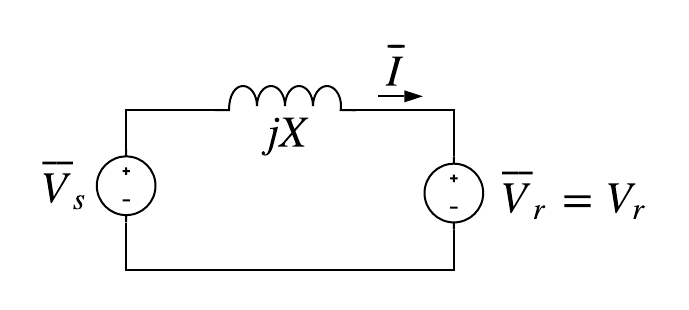
\includegraphics[width=\textwidth]{images/power-transfer_AC.png}
            \end{figure}
        \end{column}
    \end{columns}
    Let $\delta$ be the angle between $\bar{V}_r$ and $\bar{V}_s$, then
    $$
    \begin{aligned}
    S_r &= \bar{V}_r\bar{I}^* = V_r \left(\frac{V_s \angle -\delta - V_r}{-jX}\right) \\
         &= \frac{V_s V_r \sin \delta }{X} +j \frac{V_s V_r \cos \delta - V^2_r}{X}
    \end{aligned}
    $$
    \textbf{Let's remember two things:}
    \begin{itemize}
        \item The \textbf{active} power is highly sensitive to \textbf{$\delta$}
        \item The \textbf{reactive} power acts on the \textbf{voltage magnitude} (look at what happens for $\delta=0$)
    \end{itemize}

\end{frame}


\begin{frame}{Illustration \href{https://colab.research.google.com/drive/1wrJYI082Y6qE6TyaT5a7eWO1lB0CCWiu?usp=sharing}{\textcolor{blue}{\underline{(link to Python notebook)}}}
}
\begin{center}
    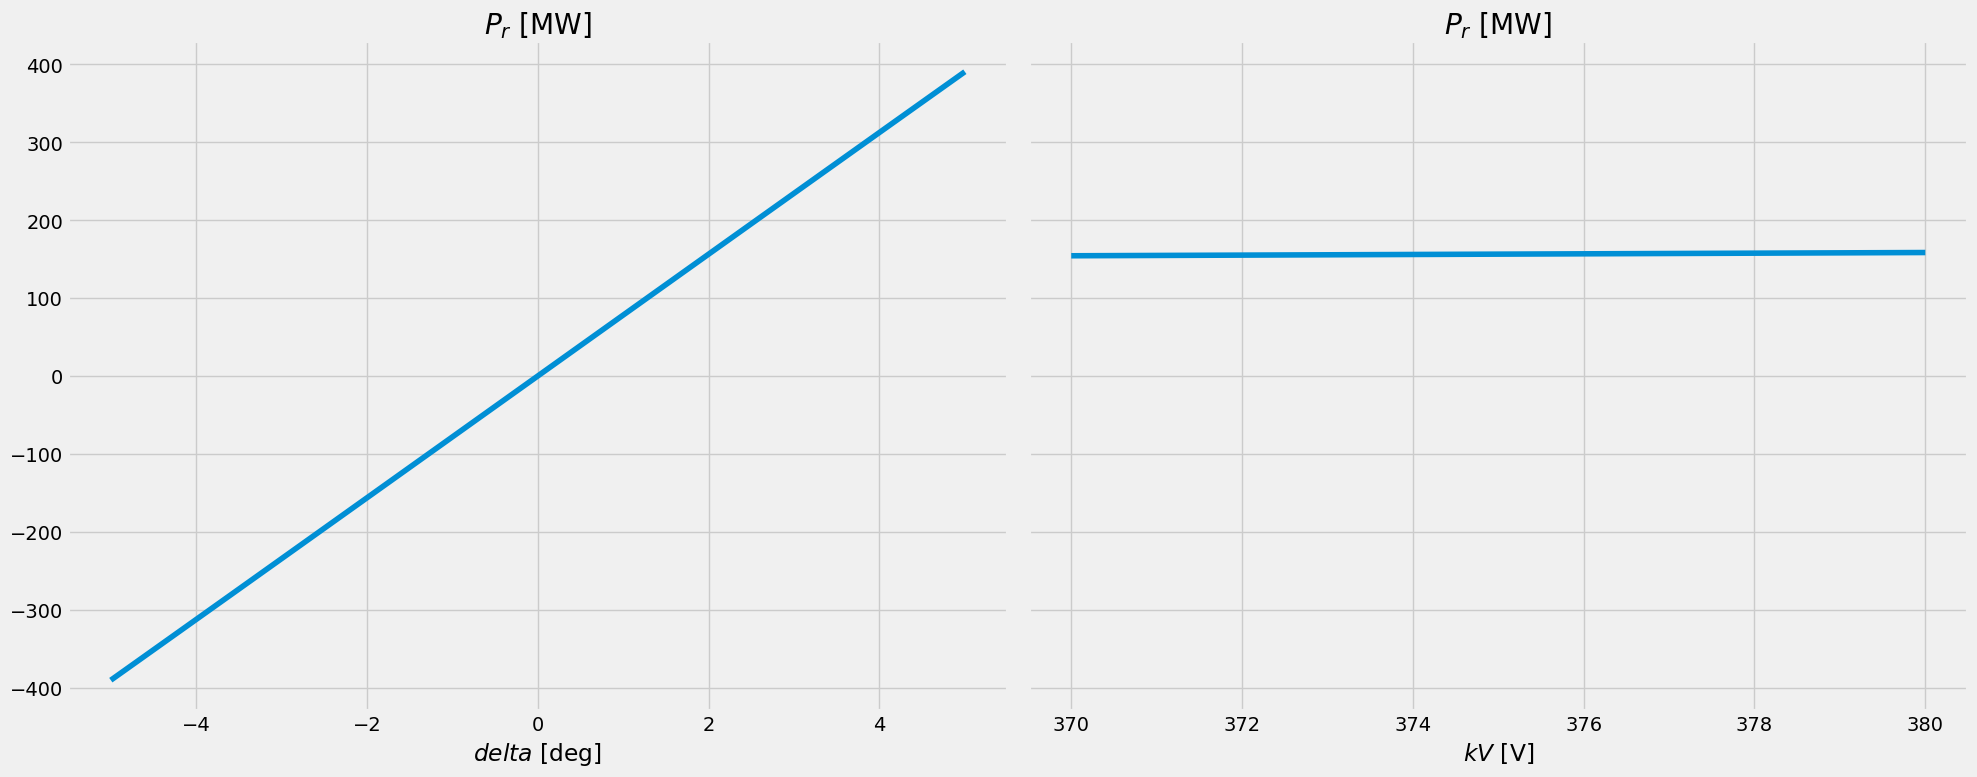
\includegraphics[width=\textwidth]{images/P_transfer.png}
\end{center}
    

\end{frame}

% Per-unit normalization slide
\section{Per-unit normalization}

% Per-unit values slide
\begin{frame}{Per-unit values}
    Per-unit values are the ratio between the actual value and the base value.
    $$
    \text{Value}_{pu} = \frac{\text{Actual value}}{\text{Base value}}
    $$
    It is useful in electrical power systems for two reasons:
    \begin{itemize}
        \item The parameters of rotating machines and transformers provided by the manufacturers are often given in pu.
        \item In a transformer, the impedance (in ohm) changes according to the square of the voltage ratio. If we express the impedance in pu, the value is invariant from one side of the transformer to the other.
    \end{itemize}
    In an electric network, a single base power is sufficient for the whole system, but for a system with transformers, one base voltage per voltage level is preferable.
\end{frame}

\begin{frame}{Working in per unit in 5 steps}
\begin{enumerate}
    \item Chose 3\footnote{When there are transformers, one base voltage per voltage level is preferrable} "fundamental" base values:
    \begin{itemize}
        \item $V_B$ for the voltage $[\mathrm{kV}]$
        \item $S_B$ for the power [MVA]
        \item $t_B$ for the time $[\mathrm{s}]$, or $\omega_B$ for the angular frequency $[\mathrm{rad} / \mathrm{s}]$
    \end{itemize}
    \item Derive other needed base values from physical laws, e.g.
    \begin{itemize}
        \item the base current: $I_B=S_B / V_B$ [A]
        \item the base impedance: $Z_B=V_B^2 / S_B[\Omega]$
    \end{itemize}
    \item Normalize input data: divide parameters by their base value
    \item Make your computations
    \item (If necessary) Apply the inverse transformation
\end{enumerate}

Data in per unit is by definition dimensionless; pay attention to base value units w.r.t. to physical value units!
\end{frame}

% Example slide
\begin{frame}[allowframebreaks]{Example}
    It is \textbf{known} that the internal reactance of a synchronous machine lies typically in the range $[1.5, 2.5] \text{ pu}$ (on the machine base)! 
     
    A machine with the characteristics $(20 \text{ kV}, 300 \text{ MVA})$ has a reactance of $2.667 \ \Omega$.\\ Is this a normal value?
    \begin{itemize}
        \item (Here we do not need a base value for time)
        \item The base impedance is $Z_B = 20^2/300 = 1.333 \ \Omega$
        \item Hence the value of the reactance in per unit is $2.667/1.333 = 2 \ pu$
        \item This is a quite normal value!
    \end{itemize}
    Same question for a machine with the characteristics $(15 \text{ kV}, 30 \text{ MVA})$
    \begin{itemize}
        \item The base impedance is now $Z_B=15^2/30 = 7.5 \ \Omega$
        \item The value of the reactance in per unit is $2.667/7.5 = 0.356 \ pu$
        \item Hence an abnormal small value!
    \end{itemize}
\end{frame}

% Per unit in three-phase systems slide
\begin{frame}{Per unit in three-phase systems}
    Let the base power $S_B$ be the three-phase power, and $U_b=\sqrt{3}V_B$ be the line to line voltage base.

    The (single-phase) base current is $$I_B = \frac{S_B}{3V_B} = \frac{S_B}{\sqrt{3}U_B}$$

    The base impedance is $$Z_B = \frac{V_B}{I_B} = \frac{3V^2_B}{S_B} = \frac{U_B^2}{S_B}$$

    In a single phase equivalent representation, the power values in per unit can be multiplied by $S_b$ to get the total three-phase power.
\end{frame}
  
\end{document}
\section{Common coordinate transformations}

\begin{frame}{Motivation}
    As a power system engineer, you will frequently encounter a few coordinate transformations.

    They serve different goals:
    \begin{itemize}
        \item Analyse \textbf{unbalanced faults} and design \textbf{protection relays}
        \item Simplify the analysis and design of \textbf{controllers}, such as proportional-integral-derivative (PID) controllers in generators or motors.
    \end{itemize}

\end{frame}

\subsection{Symmetrical components}

\begin{frame}[allowframebreaks]{The symmetrical components}

The symmetrical components transformation is also called the Fortescue transformation, named after Charles LeGeyt Fortescue (1876–1936).

It is useful for analysing unbalanced three-phases systems, such as systems where loads are unbalances, or when unbalanced faults occur:

\begin{center}
    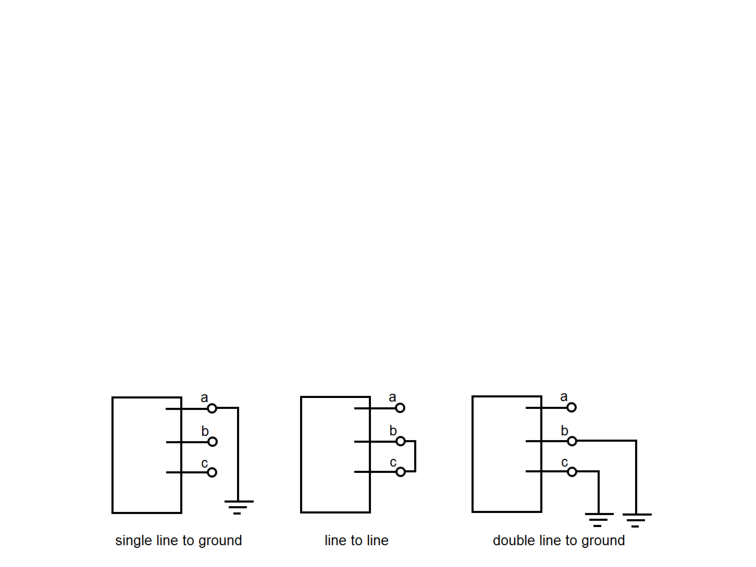
\includegraphics[width=0.6\textwidth]{images/faults.pdf}
\end{center}


Consider a set of three-phase \textbf{unbalanced} voltages $\bar{V}_{ga}, \bar{V}_{gb}, \bar{V}_{gc}$ (it applies equally to currents). 
Let's focus on $\bar{V}_{ga}$. 
The symmetrical component transformations states that it is possible to decompose $\bar{V}_{ga}$ into
$$\bar{V}_{ga} = \bar{V}_{g0} + \bar{V}_{g1} + \bar{V}_{g2} $$
where 
\begin{itemize}
    \item $\bar{V}_{g1}$ is a \textbf{direct (or positive)} sequence phasor
    \item $\bar{V}_{g2}$ is an \textbf{inverse (or negative) sequence} phasor
    \item $\bar{V}_{g0}$ is a \textbf{zero sequence} phasor
\end{itemize}

Let $a = e^{j\frac{2\pi}{3}} = 1\angle 120^{\circ}$.
Since, in the case of balanced voltages, we have $\bar{V}_{gb} = a^2 \bar{V}_{ga}$ and $\bar{V}_{gc} = a \bar{V}_{ga}$, 
we can write for the case of unbalanced voltages 
$$\bar{V}_{gb} = \bar{V}_{g0} + a^2 \bar{V}_{g1} + a \bar{V}_{g2}$$
and 
$$\bar{V}_{gc} = \bar{V}_{g0} + a \bar{V}_{g1} + a^2 \bar{V}_{g2}$$
This transformation be summarized in matrix form to 
\begin{align}
\left[\begin{array}{l}\bar{V}_{ga} \\ \bar{V}_{gb} \\ \bar{V}_{gc}\end{array}\right]
    & =\left[
    \begin{array}{ccc}1 & 1 & 1 \\ 
    1 & a^2 & a \\ 
    1 & a & a^2
    \end{array}\right]
    \left[\begin{array}{l}\bar{V}_{g0} \\ \bar{V}_{g1} \\ \bar{V}_{g2}\end{array}\right] \\
    & = \mathbf{T} \left[\begin{array}{l}\bar{V}_{g0} \\ \bar{V}_{g1} \\ \bar{V}_{g2}\end{array}\right]
\end{align}

The inverse transformation is 
\begin{align}
\left[\begin{array}{l}\bar{V}_{g0} \\ \bar{V}_{g1} \\ \bar{V}_{g2}\end{array}\right]
    & = \frac{1}{3}\left[
    \begin{array}{ccc}1 & 1 & 1 \\ 
    1 & a & a^2 \\ 
    1 & a^2 & a
    \end{array}\right]
     \left[\begin{array}{l}\bar{V}_{ga} \\ \bar{V}_{gb} \\ \bar{V}_{gc}\end{array}\right] \\
    & = \mathbf{T}^{-1} \left[\begin{array}{l}\bar{V}_{ga} \\ \bar{V}_{gb} \\ \bar{V}_{gc}\end{array}\right]
\end{align}
\end{frame}


\begin{frame}{Illustration}

See Python code (collab) TODO    

\end{frame}

\begin{frame}{Exercise}

Compute symmetrical components in one specific case of $$\left[\begin{array}{l}\bar{V}_{g0} \\ \bar{V}_{g1} \\ \bar{V}_{g2}\end{array}\right]$$ ?
Is it useful ? 

\end{frame}


\begin{frame}[allowframebreaks]{Usage of symmetrical components}

In a \textbf{balanced} system, 
\begin{itemize}
    \item \alert{positive-sequence} currents flowing create \textbf{only} \alert{positive-sequence} voltage drops 
    \item \alert{negative-sequence} currents flowing create \textbf{only} \alert{negative-sequence} drops 
    \item \alert{zero-sequence} currents flowing create \textbf{only} \alert{zero-sequence} voltage drops 
\end{itemize}

It is not the case for an unbalanced system!  For instance, positive-sequence currents flowing \textbf{can} create positive-, negative-, and zero-sequence voltage drops. 
    
Why is it useful then? 

\begin{itemize}
    \item We can also apply the \textbf{symmectrical component transformation to network components}: loads, transmission lines, transformers, machines. 
    \item This yelds positive-, negative-, and zero-sequence networks
    \item These networks can be combined at the location of fault, and as a function of the fault type (we will not detail this)
    \item From the resulting network, we can compute the symmetrical components voltages and currents. 
    \item We can apply the inverse transform to get back the current and voltage phasors in the $abc$ frame.
    \item We can also \textbf{design protections} based on the value of the symmetrical components values! For instance, zero-sequence current is a direct indicator of a ground fault, and its detection is a standard practice for overcurrent ground fault protection.
\end{itemize}
\end{frame}

\subsection{The $dq0$ Transformation}
% Frame 1: The dq0 Transform
\begin{frame}{The $dq0$ Transformation}

The $dq0$ transformaion converts three-phase ($abc$) quantities into a new $dq0$ frame.
The goal is to simplify analysis and control of AC machines and converters

\textbf{Why is it useful?}
\begin{itemize}
    \item It transforms time-varying sinusoidal quantities into constant DC quantities in a rotating reference frame.
    \item This removes the time-varying coefficients from the differential equations describing the system, making them much easier to solve.
    \item Ideal for real-time control, as it eliminates the need for complex trigonometric calculations.
\end{itemize}
\end{frame}

% Frame 2: The Clarke Transform
\begin{frame}[allowframebreaks]{The Clarke Transform ($\alpha\beta0$)}

The Clarke transform is the first step in the $dq0$ transform:
\begin{itemize}
    \item It converts a three-phase system ($a,b,c$) into a two-phase orthogonal stationary system ($\alpha, \beta$), and a zero-sequence component ($0$).
    \item The $\alpha$-axis is aligned with the $a$-phase axis.
\end{itemize}

The Clarke transform matrix is:
    $$
    T_{abc \to \alpha\beta0} = \begin{bmatrix}
    \frac{2}{3} & -\frac{1}{3} & -\frac{1}{3} \\
    0 & \frac{\sqrt{3}}{3} & -\frac{\sqrt{3}}{3} \\
    \frac{1}{3} & \frac{1}{3} & \frac{1}{3}
    \end{bmatrix}
    $$

The transformed quantities are:
    $$
    \begin{bmatrix}
    V_\alpha \\ V_\beta \\ V_0
    \end{bmatrix} = T_{abc \to \alpha\beta0} \begin{bmatrix}
    V_a \\ V_b \\ V_c
    \end{bmatrix}
    $$
\end{frame}

% Frame 3: The Park Transform
\begin{frame}[allowframebreaks]{The Park Transform ($dq$)}

The second step in the $dq0$ transform is the Park Transform, named after Robert H. Park (1902 – 1994): 
\begin{itemize}
    \item It converts the stationary $\alpha\beta$ quantities from the Clarke transform into a rotating $dq$ reference frame.
    \item This frame rotates at the same speed as the synchronous machine's rotor or the fundamental frequency of the system.
\end{itemize}

The Park transform matrix is:
    $$
    T_{\alpha\beta \to dq} = \begin{bmatrix}
    \cos(\theta) & \sin(\theta) \\
    -\sin(\theta) & \cos(\theta)
    \end{bmatrix}
    $$
The transformed quantities are:
    $$
    \begin{bmatrix}
    V_d \\ V_q
    \end{bmatrix} = T_{\alpha\beta \to dq} \begin{bmatrix}
    V_\alpha \\ V_\beta
    \end{bmatrix}
    $$
Note: $\theta$ is the angle of the rotating frame with respect to the stationary $\alpha$-axis.
\end{frame}

% Frame 4: Summary and Flow
\begin{frame}{Summary of the $dq0$ Transform}

\textbf{Complete Transformation Flow:}
\begin{enumerate}
    \item \textbf{Clarke Transform:} Transform $V_{abc}$ to $V_{\alpha\beta0}$. This is a simple change of basis from a three-phase to a stationary two-phase system.
    \item \textbf{Park Transform:} Transform $V_{\alpha\beta}$ to $V_{dq}$. This is a rotation of the reference frame, which locks onto the synchronous machine's rotor position or the phase of the system.
\end{enumerate}

\textbf{Result:}
\begin{itemize}
    \item The sinusoidal three-phase quantities are converted to constant DC quantities in the $dq$ frame.
    \item This simplifies the machine equations, enabling linear and decoupled control.
\end{itemize}
\end{frame}